\chapter{IDEA DR calorimeter full simulation}
As already said, the concept described in chapter \ref{chap:Idea_project} is an on-going project and it has to be supported by simulation.
With this goal, a dual-readout calorimeter full simulation has been developed allowing to generate data and monitor the whole process from the collision on the interaction point to the digitized signal produced by SiPMs.\\

The chapter presents a description of the simulation structure. The section \ref{sec:Sim_struc} describes in details the simulation dividing it in two main Monte Carlo processes:
\begin{itemize}
	\item the calorimeter simulation, coded in GEANT4;
	\item the SiPM response digitization (``pySIPM"), coded in Python.
\end{itemize}

Later, the performances obtained will be shown. The temporal behavior, the SiPM saturation effect and the energy resolution will be described in section \ref{sec:Sim_perf}.\\

Then the chapter treats of the possibility of simple particle identification using neural network structures.\\
%In section \ref{sec:NN_waveform} neural networks working on digitized waveforms are described. The aim of these neural network is to correctly distinguish waveforms generated by electrons ($e^-$) or pions ($\pi^-$) in a range of energy from $20$ to $80$ GeV.\\
The last section (sec.\ref{sec:NN_img})  exposes a neural network that has the purpose of identify if signal are generated from photons ($\gamma$) or neutral pions ($\pi^0$). This aim is achieved analyzing the spatial pattern of energy released in the calorimeter.

\section{Simulation structure} \label{sec:Sim_struc}

\subsection{Calorimeter simulation} \label{subsec:Sim_cal}
The calorimeter simulated follows the idea show in chapter \ref{chap:Idea_project}. As can be seen, it has a cylindrical symmetry characterized by a barrel and two endcaps. This $4\pi$ structure is obtained rotating $36$ simpler component, called slices, around the $z$ axis. The dimensions of the slices are shown in figure \ref{fig:cal_slices}, therefore the inner diameter and  the inner length are both $5\ m$ meanwhile the overall outer diameter and length are $9\ m$.\\
Each half slice is composed by 75 $2\ m$ long towers ($40$ part of the barrel and $35$ part of the endcap), $5400$ of this element are used to set up the whole calorimeter.
To correctly cover an almost $4\pi$ solid angle each tower has different trapezoidal inner face with dimensions that can vary from $\sim 5\ cm$ to $\sim 8\ cm$.
A small circular area, with $0.25\ m$ of radius, centered along the $z$ axis is not covered by the calorimeter to permit the beam to reach the interaction point (IP).\\

\begin{figure}
	\centering
	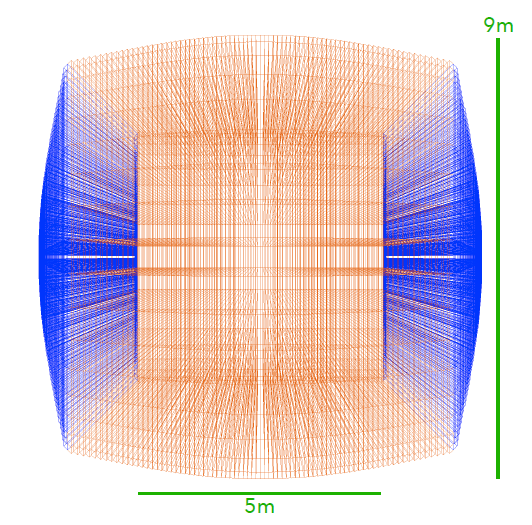
\includegraphics[width=0.6\textwidth]{IMG/DRCGeometry3}
	\caption{Calorimeter geometry.}
	\label{fig:cal_geometry}
\end{figure}
\begin{figure}
	\centering
	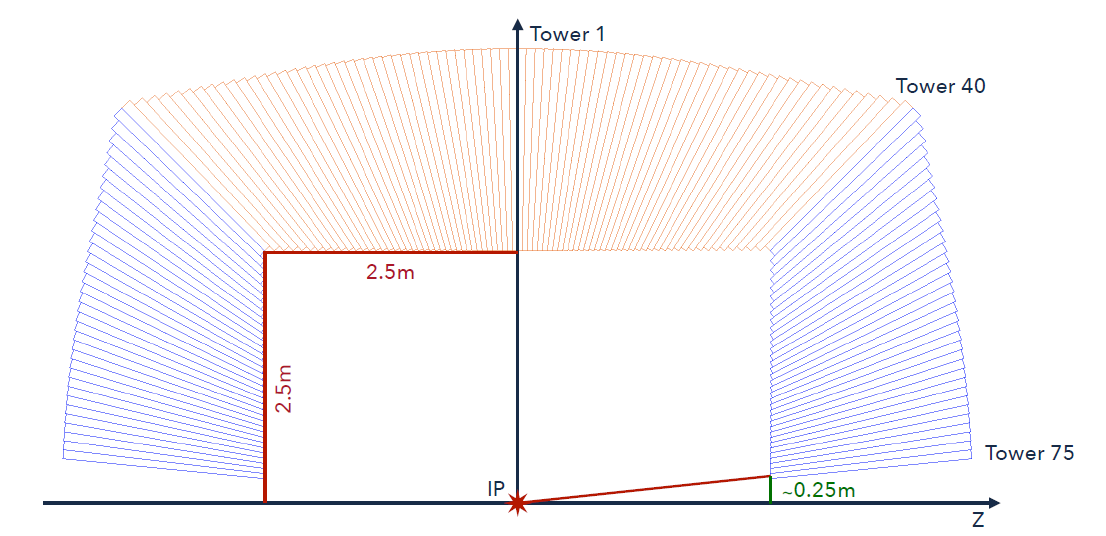
\includegraphics[width=0.8\textwidth]{IMG/DRCGeometry1}
	\caption{Calorimeter single slice.}
	\label{fig:cal_slices}
\end{figure}

The towers are copper based and play the role of absorber. To have a sensitive element they are filled by optical fibres. The idea of a projective calorimeter make the absorber volume greater increasing the distances from the IP. New fibres at different depth have to be placed inside the calorimeter to keep constant the sampling fraction.\\
As the dual-readout technique needs to distinguish Scintillating ($S$) and Cherenkov ($C$) signal, two types of fibres are used (fig. \ref{fig:CS_fibres}). Their characteristic are shown in tab. \ref{tab:fibres}.\\
The fibre refractive indices determine the light transport (as consequence of the Snell's law \cite{Snell}). The signal from the scintillating fibres is parametrised by the deposited energy while the Cherenkov photons are produced accordingly to the Cherenkov emission process.\\

\begin{table}
	\centering
	\setlength{\tabcolsep}{12pt}
	\begin{tabular}{lp{0.6\textwidth}}
		\toprule
		\multicolumn{2}{c}{\textbf{Kuraray SCSF-78 ($S$)}}	\\
		\midrule
		Core:				& $r = 0.485\ mm$, Polystyrene ($C_5H_5$), $\rho=1.95\ g/cm^3$, $n = 1.59$	\\
		Cladding: 			& Thickness $=2\%$ of $r$, PMMA ($C_5H_8o_2$), $\rho=1.19\ g/cm^3$, $n=1.49$	\\
		Main properties:	& Emission constant $= 2.8\ ns$, LY $= 10^4\ \text{photons}/MeV$, $\lambda_{att} = 4\ m$	\\
		\midrule
		\multicolumn{2}{c}{\textbf{Mitsubishi SK-40 ($C$)}}	\\
		\midrule
		Core:				& $r = 0.485\ mm$, PMMA ($C_5H_8o_2$), $\rho=1.19\ g/cm^3$, $n = 1.49$	\\
		Cladding: 			& Thickness $=2\%$ of $r$, Fluorinated Polymer ($C_2F_2$), $\rho=1.43\ g/cm^3$, $n=1.42$	\\
		Main properties:	& $\lambda_{att} = 8.9\ m$	\\
		\bottomrule
	\end{tabular}
	\caption{fibres $S$ and $C$.}
	\label{tab:fibres}
\end{table}

\begin{figure}
	\centering
	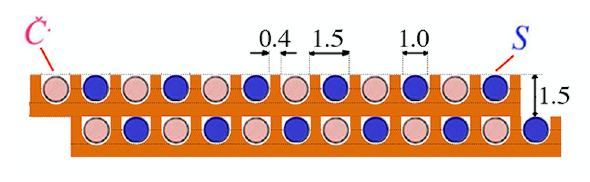
\includegraphics[width=0.8\textwidth]{IMG/DRCGeometry2}
	\caption{Fibres $C$ and $S$.}
	\label{fig:CS_fibres}
\end{figure}

For each event, the simulation gives as output useful information: 
\begin{itemize}
	\item Event ID;
	\item Fibre Type;
	\item Fibre ID;
	\item the position of the fibre end closer to the IP;
	\item the number of photons reaching the fibre further end;
	\item the list of photons time of arrival to the fibre end.
\end{itemize}

The computation of light propagation is extremely time consuming, so that it has to be fine tuned to optimize the process. In particular, the propagation of $C$ photons is tracked until the single photon reach the core-cladding boundary (i.e. at the distance $R$ from the further end of the fibre and at the time $t_0$). If the emission angle is inside the range of the fibre numerical aperture, the photon is added to the final number of photons (after a Poissonian smearing on their number).
The time of arrival on the sensor for each photon is estimated as:
\begin{equation}
t_C = t_0 + R \frac{n_C}{c}
\end{equation}
where $n_C = 1.49$ is the fibre refractive index and $c$ is the speed of light.\\

The $S$ fibres, instead, carry scintillating photons produced considering the light yield of the fibres and the energy deposited by the interacting particle. The number of photons is smeared with as Poissonian law and de time of arrival on the sensor is obtained as:
\begin{equation}
	t_S = t_0 + R\frac{n_S}{c\times \cos(\vartheta)} + t^*
\end{equation}
where $n_S = 1.59$ is the refractive index and $t^*$ is a random time that considers the fibres decay time, it is chosen from an exponential distribution with $2.8\ ns$ as mean value.
Considering the internal reflection, the photon path depends on the $\vartheta$ angle (i.e. the angle between the photon direction and the fibre axis). It is chosen randomly in the range $[\cos(\alpha),\cos(0)]$, where $\alpha = 20.4\degree$ is the fibre critical angle.\\
Eventually, the light produced is smeared by two Poissonian distribution, one for scintillation photo-electrons and the other one for Cherenkov photo-electrons. This procedure correctly reproduces statistic fluctuations in scintillation and Cherenkov light production and allows to reproduce within simulations the scintillating light yield (p.e./GeV) desired. To make the full simulation lighter, this process also includes the attenuation due to the PDE of the simulated SiPMs. The simulation is tuned to produce $\sim 400\ Spe/GeV$ and $\sim 100\ Cpe/GeV$ at the electromagnetic scale.

\subsection{SiPM response digitization} \label{subsec:Sim_SiPM}
The results obtained are the input of the second part of the simulation: \textit{pySiPM}, a Monte Carlo simulation, performed mostly in Python, able to reproduce the SiPM response to a light source and replicate the waveforms recorded with a digitizer \cite{digitizer}.\\

The importance of this software goes beyond our context, but perfectly fits our needs. In particular each fibre from the calorimeter simulation is considered coupled to a single SiPM, which digitized response is simulated through \textit{pySiPM}.

The simulation allows to set most of the SiPM parameters:
\begin{itemize}
	\item \textbf{Geometrical parameters}: the sensor dimensions and the pixel pitch.
	\item \textbf{Sensor parameters}: Photon Detection Efficiency, Dark Count Rate, After-Pulse probability, Optical Cross-Talk probability.
	\item \textbf{Signal parameters}: rise time constant, decay time constant.
	\item \textbf{Waveform parameters}: time window, sampling time, integration window.
\end{itemize}

For each event and fibre, random parameters determine the photon position inside the sensor. %Meanwhile the sensor PDE is tuned to have consistent mean values of $\sim 400\ Spe/GeV$ and $\sim 100\ Cpe/GeV$ respectively for $S$ and $C$ light yield.
Meanwhile the sensor PDE is set at $100\%$ to be consistent with the smearing applied at the calorimeter simulation level.
A control stop the count of impinging photons on the same cell to a maximum one, then each element of noise is generated with the set probability.\\
The pulse generated is a combination of two exponentials characterized by the rise time constant ($\tau_{rise}$) and the decay time constant ($\tau_{fall}$), considering the different photon time of arrival ($t_S$ and $t_C$):
\begin{equation}
	y(t)= A \cdot \left( e^{-\frac{t}{\tau_{fall}}} - e^{-\frac{t}{\tau_{rise}}}\right).
	\label{form:resp_func}
\end{equation}

The total signal of each SiPM is the sum of all the signals generated from the activated cells.\\

The information given as output of the simulation are:
\begin{itemize}
	\item \textbf{Data reported from GEANT4 simulation}: event ID, type of fibre, fibre ID, fibre position;
	\item \textbf{Computated quantities}: integral, peak height, time of arrival, time over threshold, time of peak;
	\item \textbf{Digitized waveform}.
\end{itemize}

\section{Simulation performances} \label{sec:Sim_perf}

\subsection{Different configurations} \label{subsec:SiPM_conf}
The results shown in this last chapter are obtained considering different SiPM parameters configurations.\\
They have been chosen in a common parameter space identified checking the lineup of SiPMs produced by Hamamatsy \cite{SiPM_lineup}. 
Two are the parameters that has been changed in our studies: 
\begin{itemize}
	\item the decay time constant of the signal, the chosen values are $10\ ns$ and $50\ ns$;
	\item the pixel size, the chosen values are $10\ \mu m$, $15\ \mu m$ and $25\ \mu m$.
\end{itemize}

The other fixed values of parameters are listed in the table \ref{tab:SiPM_par}.\\

\begin{table}
	\centering
	\setlength{\tabcolsep}{18pt}
	\begin{tabular}{ll}
		\toprule
		\multicolumn{2}{c}{\textbf{Geometrical Parameter}}	\\
		SiPM area	& $1 \times 1\ mm^2$	\\
		\midrule
		\multicolumn{2}{c}{\textbf{Sensor Parameters}}	\\
		DCR			& $200 \ kHz$	\\
		After-Pulse	& $3\% $	\\
		Cross-Talk	& $1\% $	\\
		\midrule
		\multicolumn{2}{c}{\textbf{Signal Parameter}}	\\
		Rise time	& $1\ ns$	\\
		\midrule
		\multicolumn{2}{c}{\textbf{Waveform Parameters}}	\\
		Time window	& $500 \ ns$	\\
		Integration window	& $300 \ ns$	\\
		Sampling frequency	& $10\ GHz$	\\
		\bottomrule
	\end{tabular}
	\caption{parameter}
	\label{tab:SiPM_par}
\end{table}

An example of waveform generated is plotted in figure \ref{fig:diff_wf} where is clear the difference produced using two different decay time constant.

\begin{figure}
	\centering
	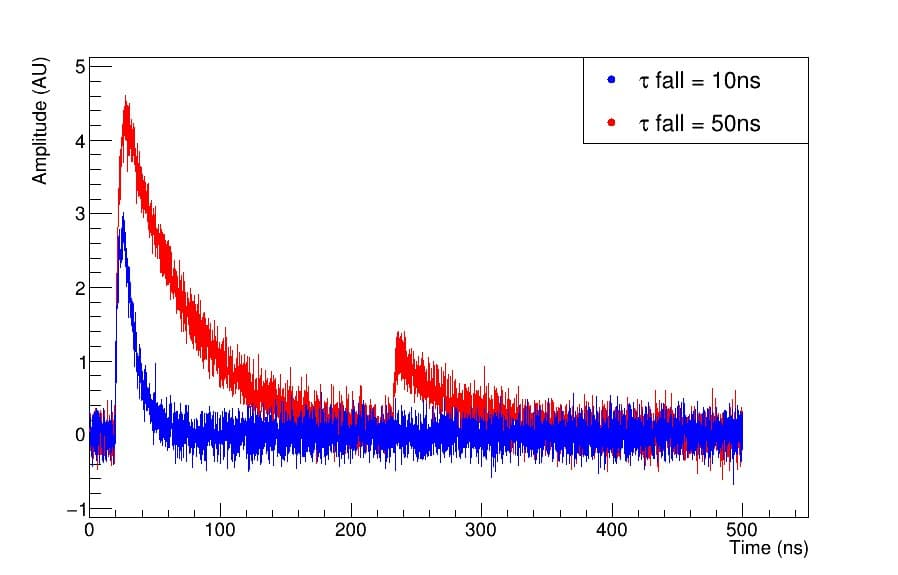
\includegraphics[width=0.8\textwidth]{IMG/SingleWaveform}
	\caption{Single waveform}
	\label{fig:diff_wf}
\end{figure}

\subsection{Time studies} \label{subsec:Time}
An important aspect that has to be studied is the temporal one.
In order to do this, data of $1000$ events are produced. In each event a $40\ GeV$ electron is produced from the interaction point.\\
A first step is to analyze the distribution of the time of arrival of the photons converted at the SiPMs (i.e. the time recorded in the GEANT4 simulation output).\\
The distribution obtained from $C$ and $S$ photons are plotted in figure \ref{fig:true_toa_dist}.
As expected, the distribution of $C$ photons time extremely narrow due to the instantaneous production of photons at the passage of relativistic charged particle in the fibres, instead the $S$ photons time distribution shows an exponential tail that is a direct consequence of the emission time constant of the Polystyrene.\\

\begin{figure}
	\centering
	\includegraphics[width=0.8\textwidth]{IMG/true_toa_dist}
	\caption{True time of arrival distribution.}
	\label{fig:true_toa_dist}
\end{figure}

Now a step forward can be done using this data as input for \textit{pySiPM}. The SiPM parameters are chosen as described in paragraph \ref{subsec:SiPM_conf}. In this context the most interesting editable parameter is the decay time constant.\\ 
Figure \ref{fig:top_50ns} and \ref{fig:top_10ns} are in analogy with respect to the last described and presents clearly a widening of the distributions, the cause of this phenomenon has to be associated to the characteristic response function of the sensors \ref{form:resp_func}.\\
These data can be compared looking for differences in changing SiPMs configurations. As we can see in figure \ref{fig:top_per_fib}, the same $C$ and $S$ photons produce narrower time of peak distribution due to the less impact of electronic noise on a sharper response function.\\

\begin{figure}
	\centering
	\subfloat[][\label{fig:top_50ns}$\tau_{fall} = 50\ ns$.]{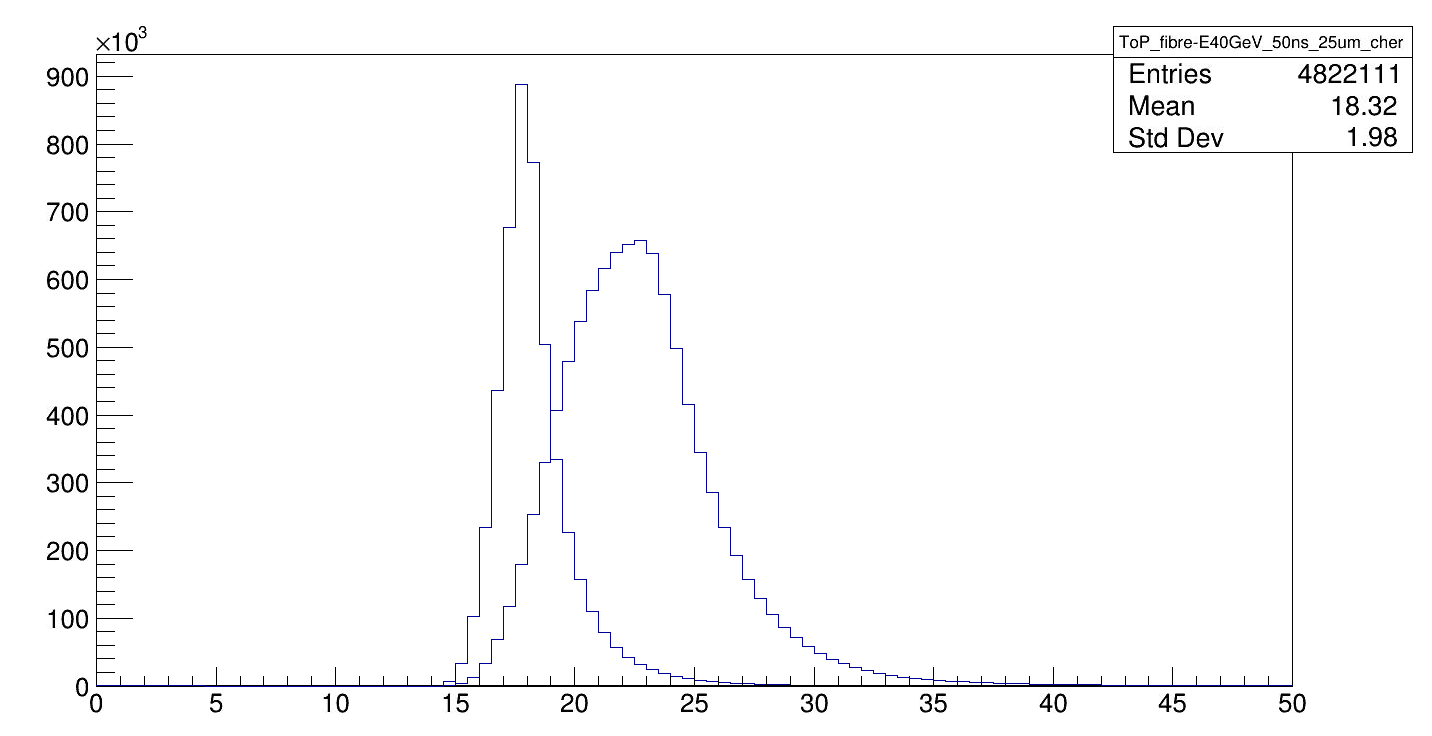
\includegraphics[width=.45\textwidth]{IMG/top_50ns}} \quad
	\subfloat[][\label{fig:top_10ns}$\tau_{fall} = 10\ ns$.]{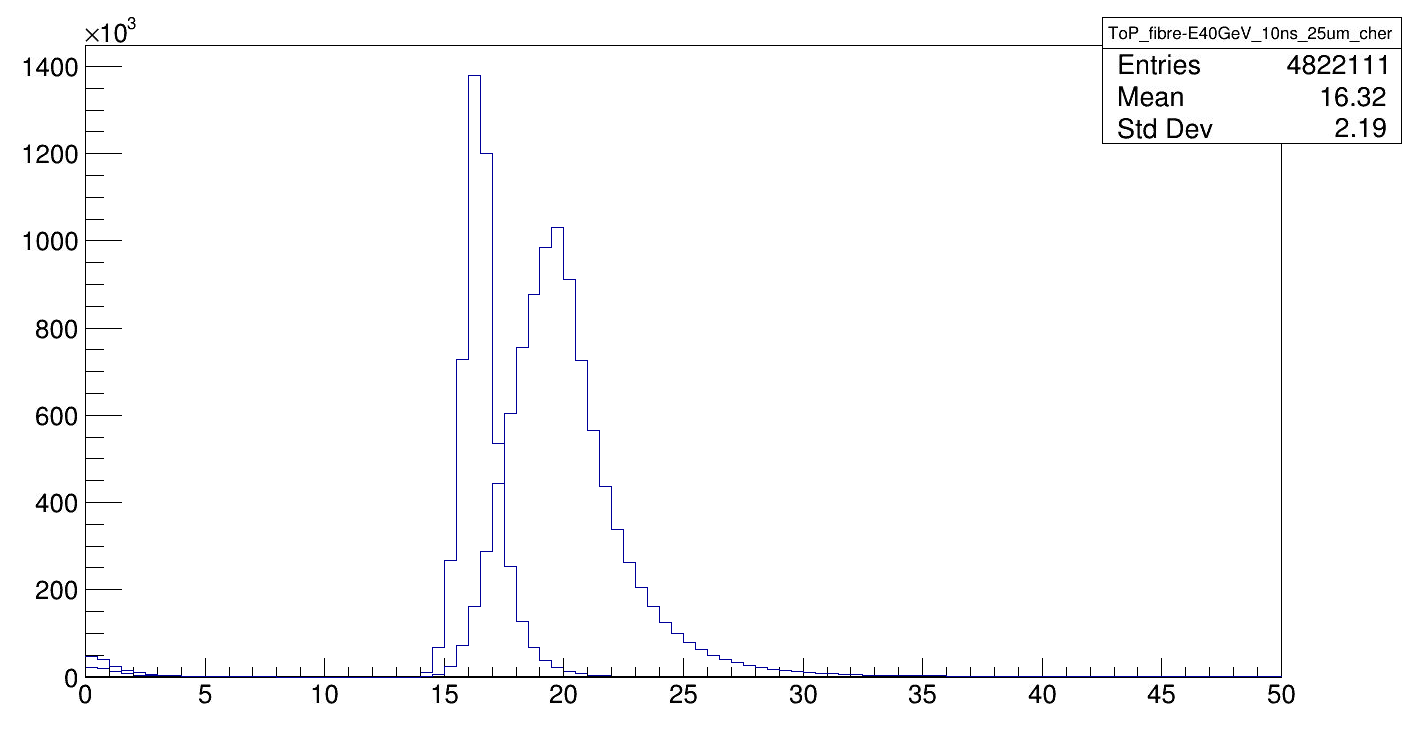
\includegraphics[width=.45\textwidth]{IMG/top_10ns}}
	\caption{time of peak distribution.}
	\label{fig:top_per_tau}
\end{figure}

\begin{figure}
	\centering
	\subfloat[][\label{fig:top_C}$C$ fibres.]{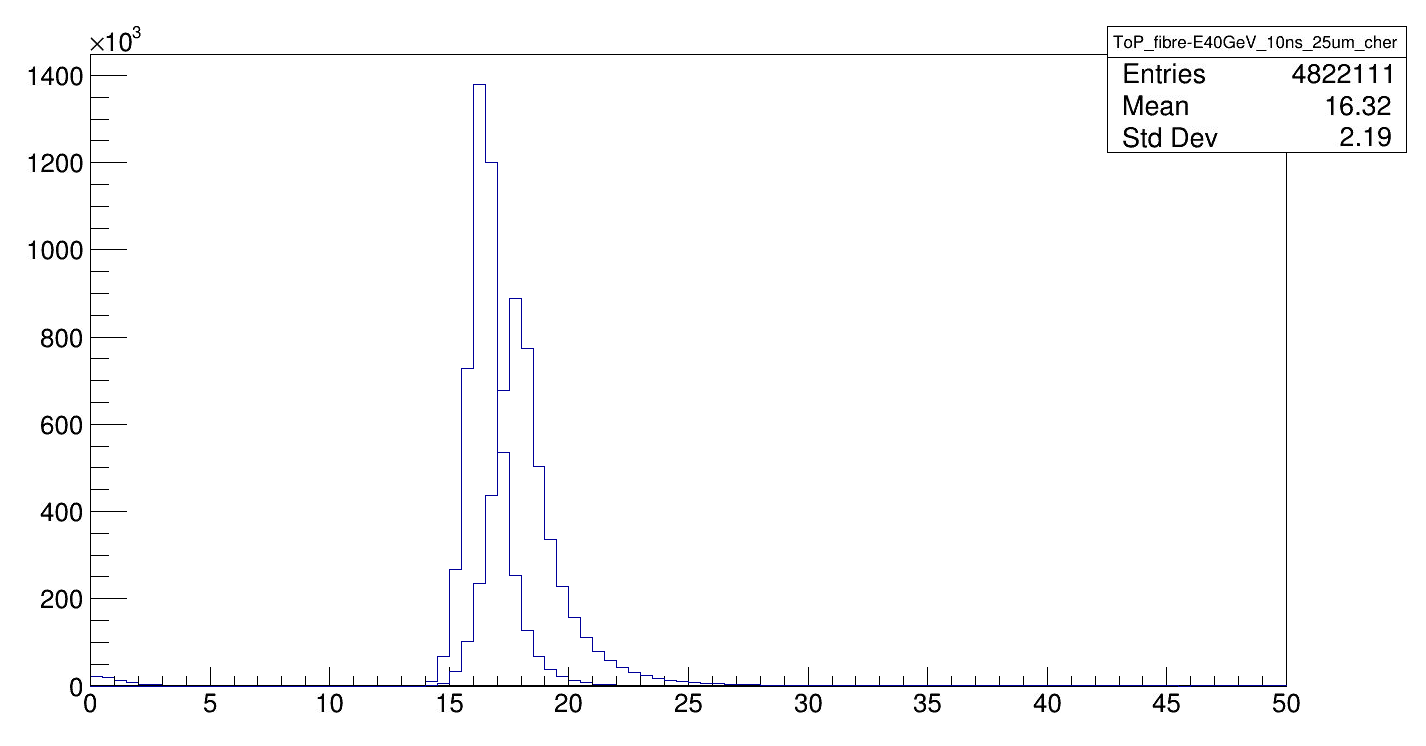
\includegraphics[width=.45\textwidth]{IMG/top_C}} \quad
	\subfloat[][\label{fig:top_S}$S$ fibres.]{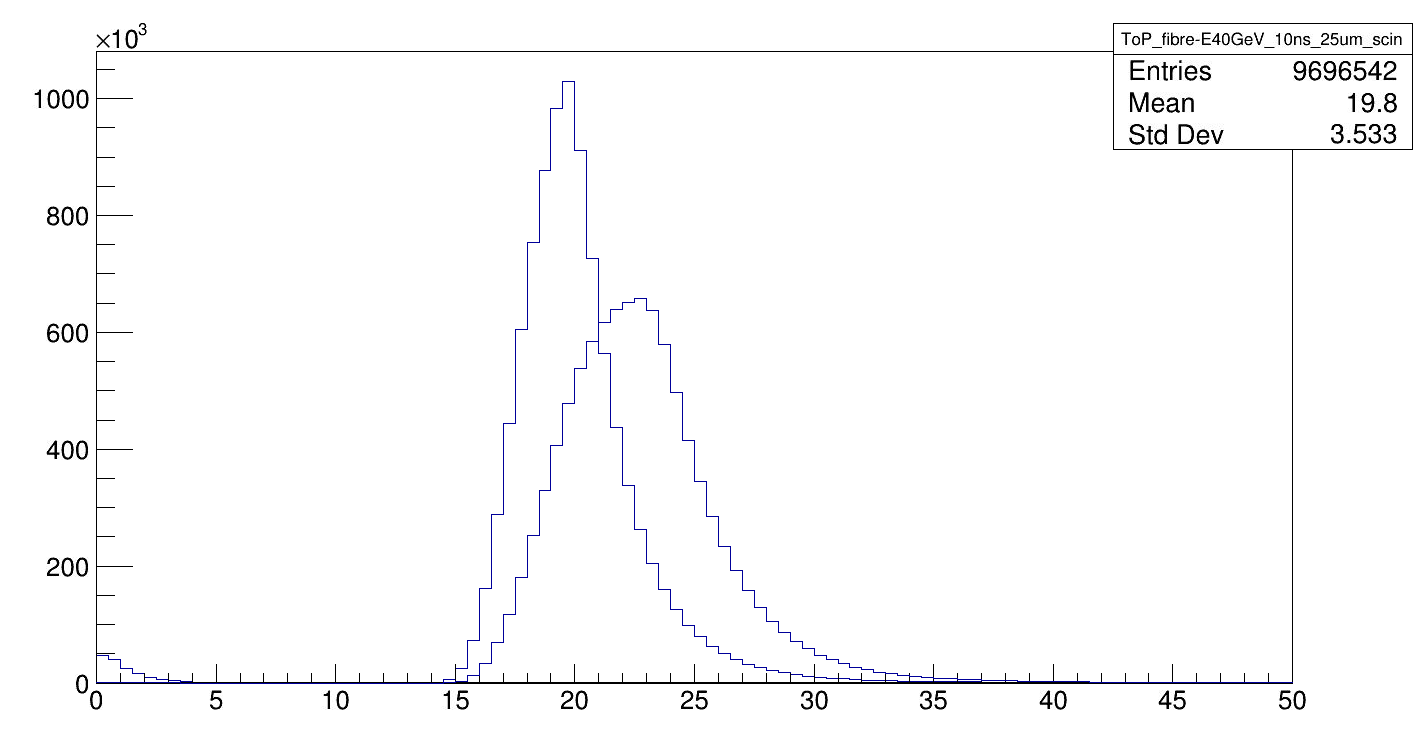
\includegraphics[width=.45\textwidth]{IMG/top_S}}
	\caption{time of peak distribution.}
	\label{fig:top_per_fib}
\end{figure}

The impact of noise on time of peak precision is also dependent on the number of photons impinging the same SiPM, in particular the peak precision increase with the number of photons.\\
To prove this $10000$ SiPMs have been fired with an increasing number of simultaneous photons. For each fixed number of photons, the time of peak has been recorded, plotted in an histogram and fitted with a Gaussian function. An example of these histograms is shown in figure \ref{fig:top_dummy}.\\

The standard deviation of these Gaussian fit is the interested quantity that has been recorded and reported in the table \ref{tab:sigmas}.\\
It is interesting to plot these data and study the behavior of the standard deviation in fuction of the number of photons. Figure \ref{fig:top_sigma} shows graphically the data, which are well fitted with a function of the form:
\begin{equation}
	\sigma = \frac{A}{\sqrt{n}} + B.
\end{equation}
The parameters obtained are $A = 0.8712\ ns$ and $B = 0.08734\ ns$ for data associated to SiPMs with $\tau_{fall}=10\ ns$, and $A = 1.949\ ns$ and $B = 0.008217\ ns$ for data associated to SiPMs with $\tau_{fall}=50\ ns$.

\begin{table}
	\centering
	\begin{tabular}{lcc}
		\toprule
		Number of photons	& $\sigma$ with $\tau_{fall}=10\ ns$ [ns] & $\sigma$ with $\tau_{fall}=50\ ns$ [ns]	\\
		\midrule
		$1$ 	& $1.4150$ & $7.0680$ \\
		$2$ 	& $0.8717$ & $2.6420$ \\
		$3$ 	& $0.6738$ & $1.7370$ \\
		$4$ 	& $0.5742$ & $1.3770$ \\
		$5$ 	& $0.5146$ & $1.1230$ \\
		$6$ 	& $0.4624$ & $0.9719$ \\
		$7$ 	& $0.4314$ & $0.9148$ \\
		$8$ 	& $0.3998$ & $0.8508$ \\
		$9$ 	& $0.3811$ & $0.7717$ \\
		$10$ 	& $0.3605$ & $0.7169$ \\
		$25$ 	& $0.2339$ & $0.4481$ \\
		$50$ 	& $0.1679$ & $0.3112$ \\
		$100$ 	& $0.1229$ & $0.2297$ \\
		\bottomrule
	\end{tabular}
	\caption{Sigmas}
	\label{tab:sigmas}
\end{table}

\begin{figure}
	\centering
	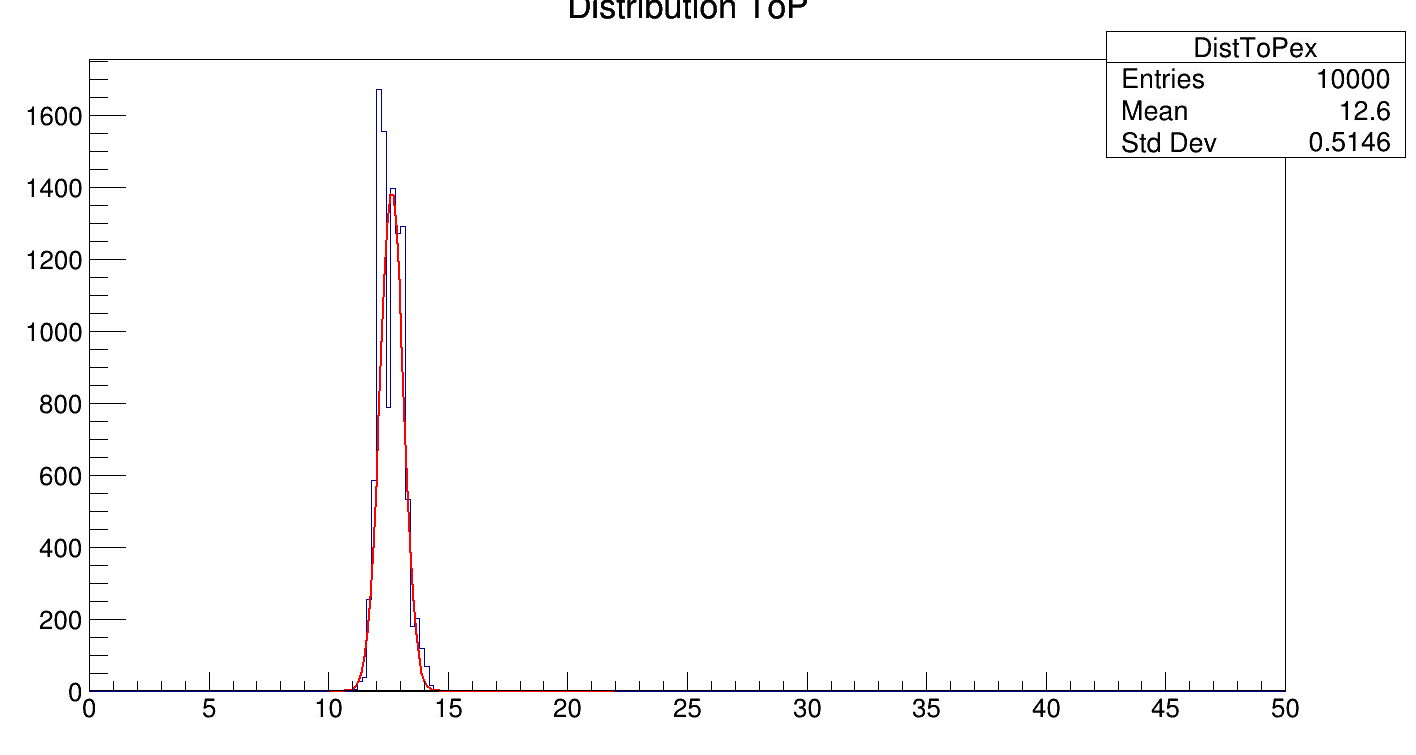
\includegraphics[width=0.8\textwidth]{IMG/top_dummy}
	\caption{Time of peak dummy, 5 photons, 50 ns.}
	\label{fig:top_dummy}
\end{figure}

\begin{figure}
	\centering
	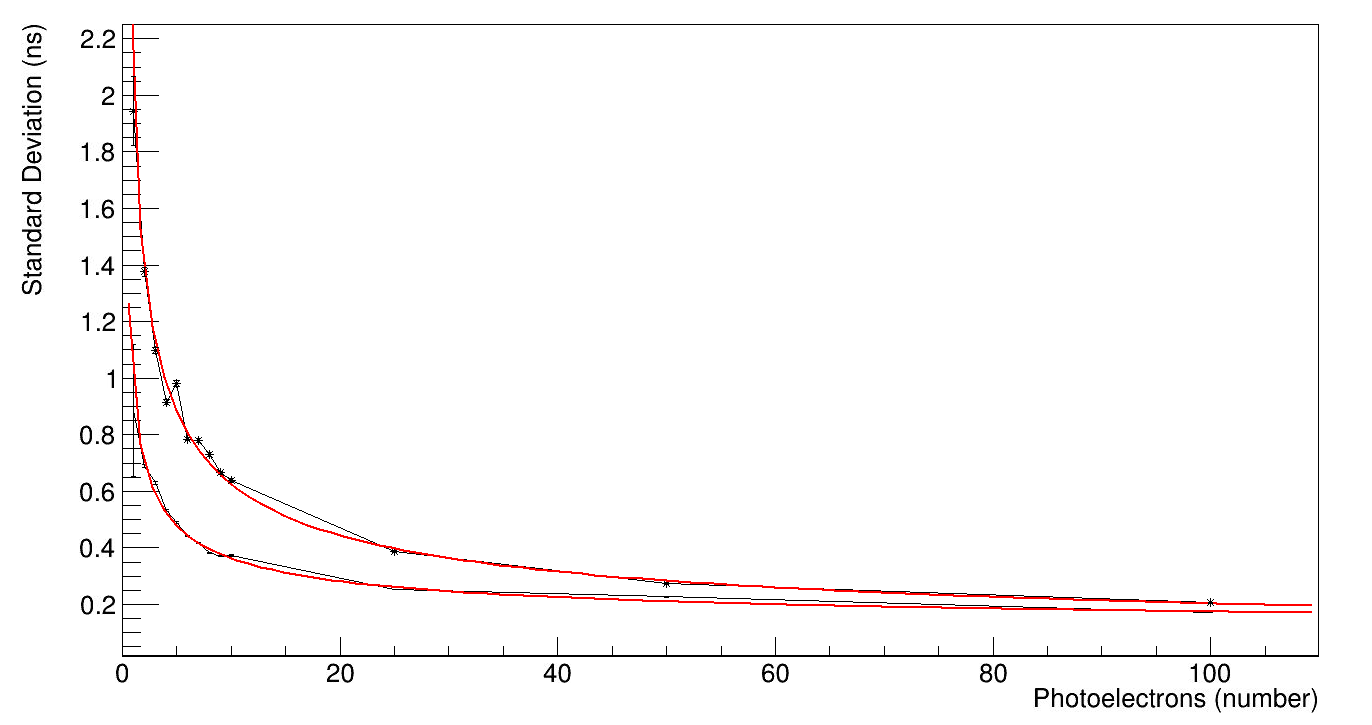
\includegraphics[width=0.8\textwidth]{IMG/top_sigma}
	\caption{Time of peak dummy, 5 photons, 50 ns.}
	\label{fig:top_sigma}
\end{figure}


\subsection{Occupancy effect} \label{subsec:Sat_effect}
The occupancy effect, as shown in the paragraph \ref{subsec:SiPM_work}, is an important characteristic that has to be deeply studied to know the behaviour of the SiPMs under high number of impinging photons and to correctly reconstruct the released energy.\\

As can be seen in figure \ref{fig:sat_example}, this effect is reproduced correctly in our simulations. The example shows the charge integral in dependence to the number of p.e. and follows the concepts already seen in paragraph \ref{subsec:occupancy_teo}.\\

\begin{figure}
	\centering
	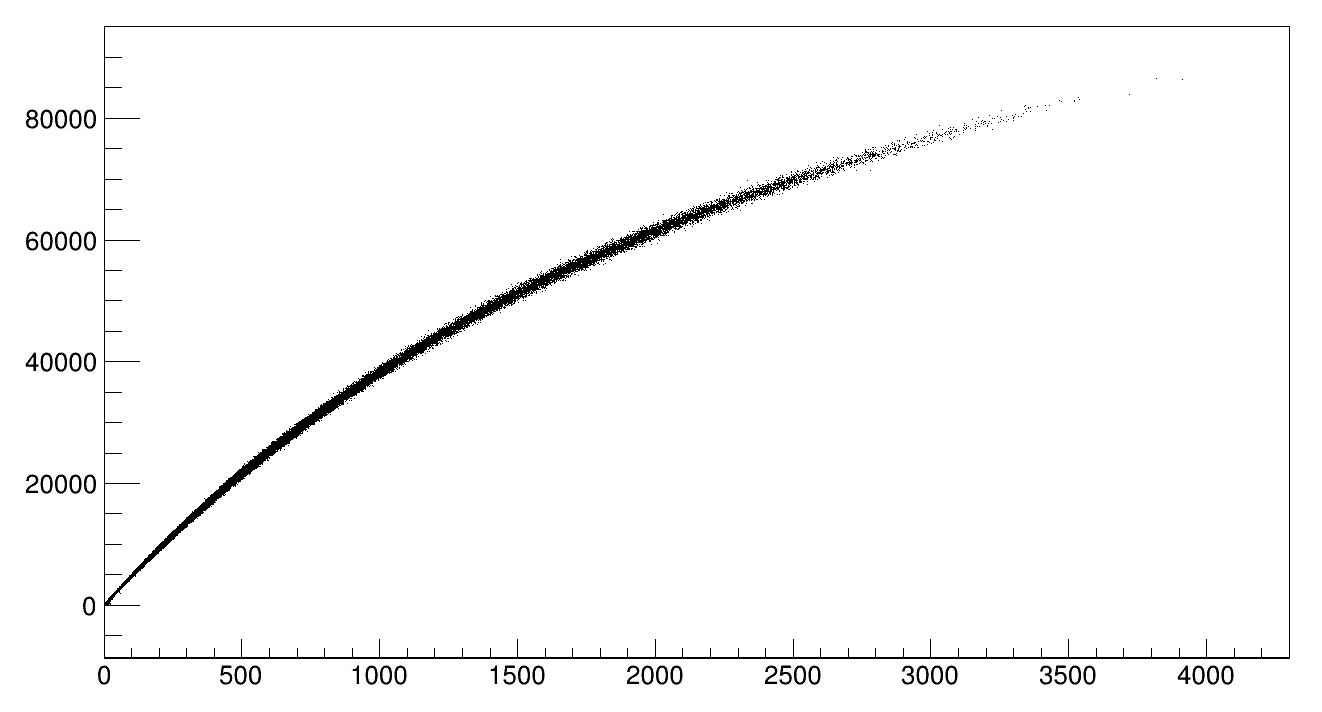
\includegraphics[width=0.7\textwidth]{IMG/Saturation_40GeV_25um_scin}
	\caption{Saturation 40GeV 25um scin.}
	\label{fig:sat_example}
\end{figure}

The first step to perform these studies is to reconstruct a calibration law that reproduces the charge integral with respect to the number of p.e. firing the same SiPM.\\
Starting by assuming that in the range of photoelectrons from $2$ to $10$ the saturation effect does not occur in our configurations (i.e. $10000$, $4356$ and $1600$ cells in each SiPM), $10000$ SiPM has been fired $9$ times with an increasing number of simultaneous p.e. in the range considered.\\
To assume that no saturation effect occurs in these data the charge integral distribution from the three different configurations has been compared finding no bias as seen in figure \ref{fig:SatCheck}. The mean and the RMS values has been recorded and fitted with a strait line corresponding to the calibration law desired:
\begin{equation}
	I(n) = A \cdot n + B
\end{equation}
with $A = 49.43 \pm 0.03852$ and $B = 2.491 \pm 0.2516$ (fig \ref{fig:NoSatLine}).\\
The parameter $A$ represents the contribution to the charge integral associated to a single photoelectron. Meanwhile $B$ is the pedestal that is originated mostly by the DCR. This contribution can be evaluated considering our parameters of DCR $= 200\ kH$ and the integration window of $300\ ns$.
$B_{DCR} = 2 \cdot 10^5 \cdot 3 \cdot 10^{-7} p.e. = 6\cdot 10^{-2} p.e. = 6\cdot 10^{-2} \cdot 49.43 = 2.96$.\\
In the following result, the value of the pedestal has been subtracted to the integral value of each SiPM.\\

\begin{figure}
	\centering
	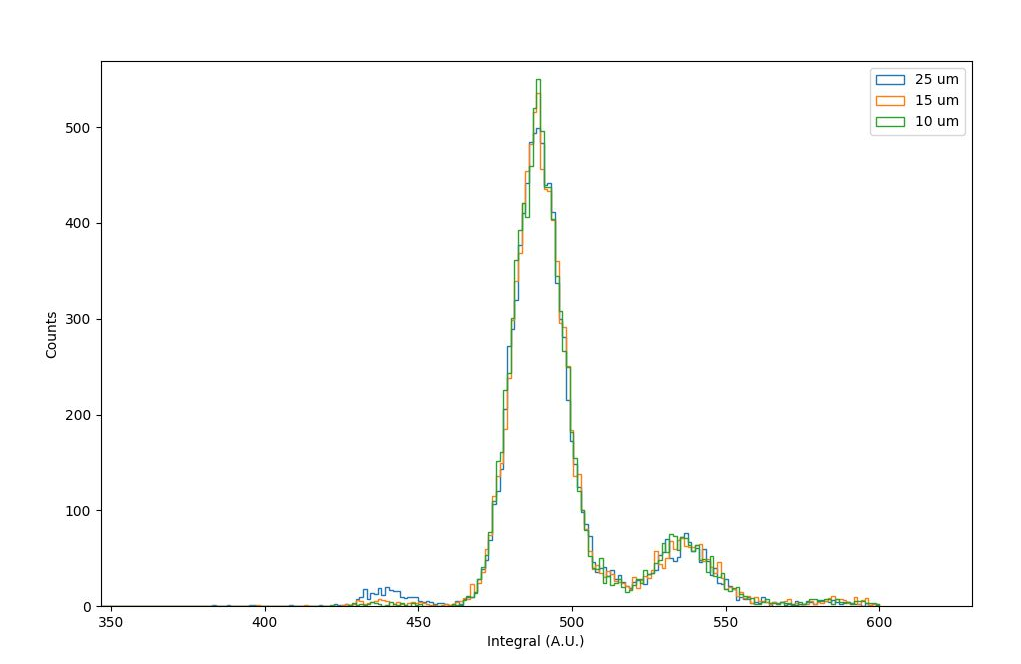
\includegraphics[width=0.7\textwidth]{IMG/10pe_sat_check}
	\caption{10pe sat check.}
	\label{fig:SatCheck}
\end{figure}

\begin{figure}
	\centering
	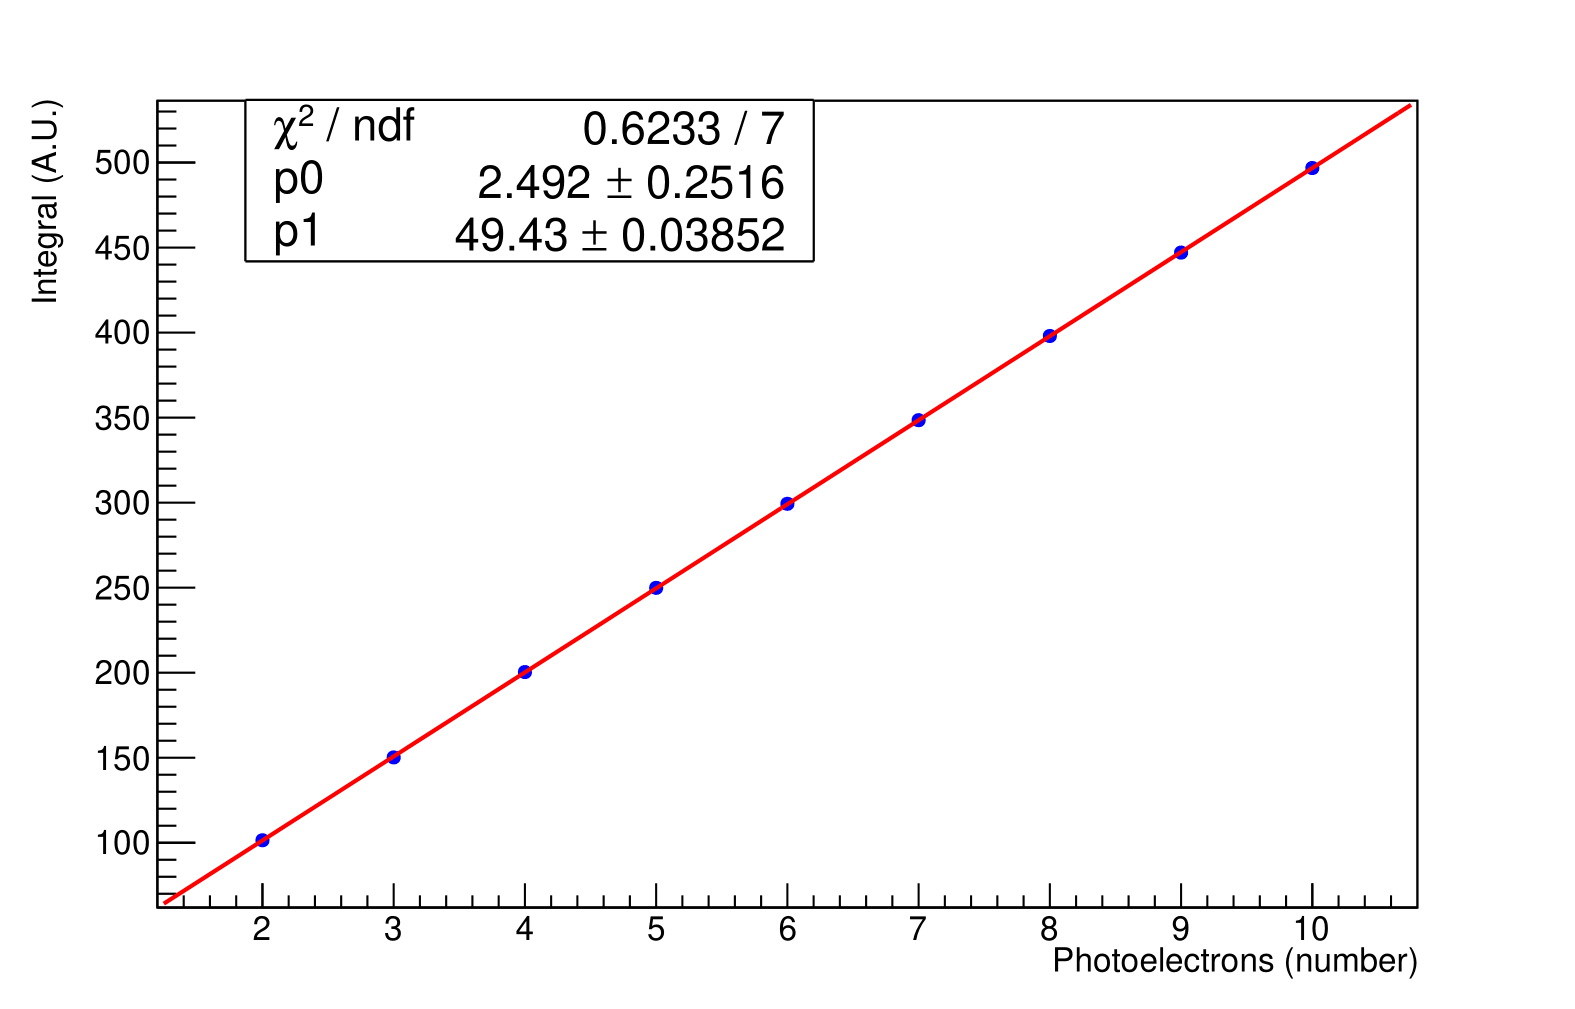
\includegraphics[width=0.7\textwidth]{IMG/NoSatLine}
	\caption{NoSatLine.}
	\label{fig:NoSatLine}
\end{figure}

The occupancy effect has been studied in electromagnetic shower produced by single electrons of different energies at each event with discrete values of $20,\ 40,\ 60,\ 80\ GeV$.\\
The impact of the saturation has been quantified using the line $I = A\cdot n$ as no saturation reference. The result obtained from $10000$ events of single $40\ GeV\ e^-$ with different SiPM configurations are separated in Cherenkov and Scintillation signals. They are shown in figure \ref{fig:sat_fibres} where each point correspond to a single SiPM. The smaller is the number of cells, the greater is the occupancy effect.\\
Moreover, as expected, the scintillation fibres transport $\sim 4$ times the p.e. from Cherenkov ones on average, therefore they are more affected to the saturation.\\

\begin{figure}
	\centering
	\subfloat[][$C$ signals.]{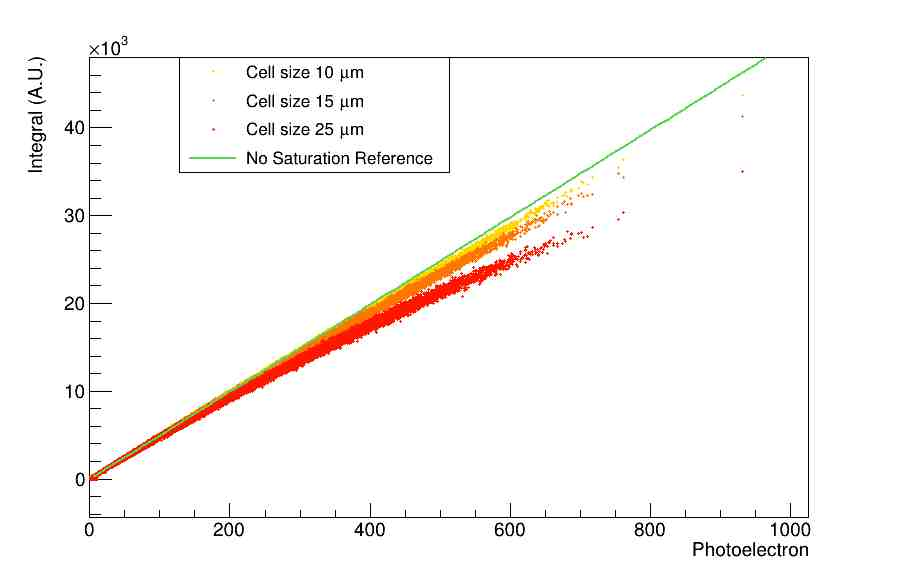
\includegraphics[width=.7\textwidth]{IMG/Sat_Fib_40GeV_cher}} \\
	\subfloat[][$S$ signals.]{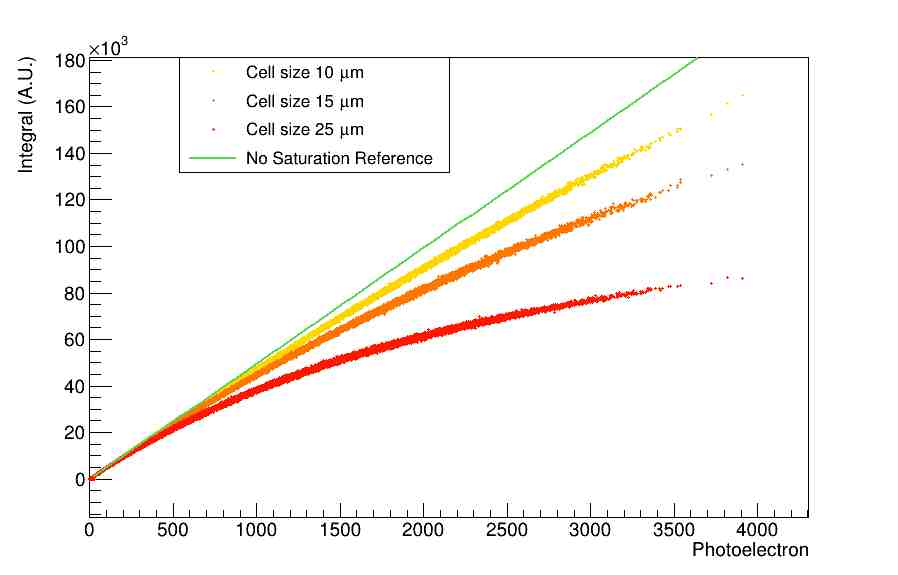
\includegraphics[width=.7\textwidth]{IMG/Sat_Fib_40GeV_scin}}
	\caption{Saturation fibres.}
	\label{fig:sat_fibres}
\end{figure}

This process can be extended considering one event at the time and adding the charge integral and the corresponding number of photoelectrons. The effect produced is represented in figure \ref{fig:sat_events} where each point correspond to a single event.\\

\begin{figure}
	\centering
	\subfloat[][$C$ signals.]{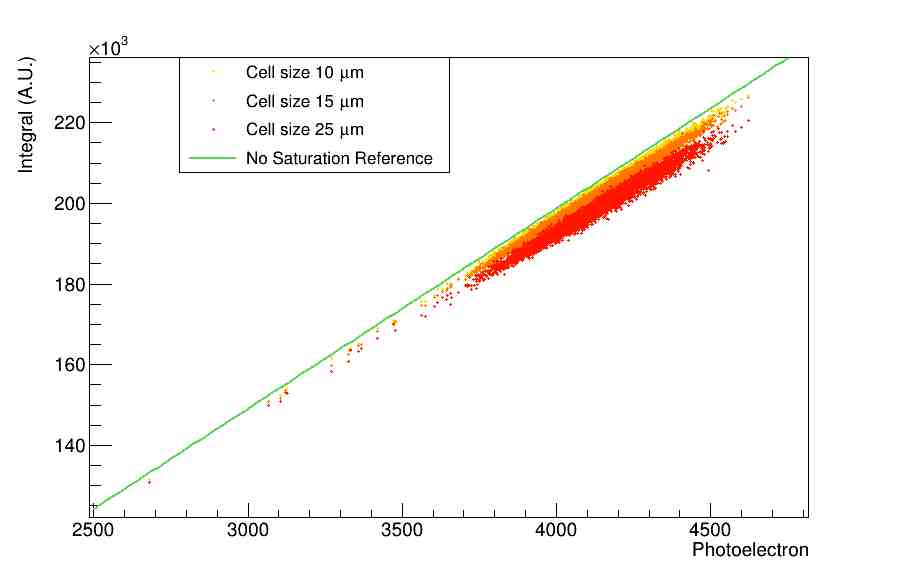
\includegraphics[width=.7\textwidth]{IMG/Sat_Ev_40GeV_cher}}\\
	\subfloat[][$S$ signals.]{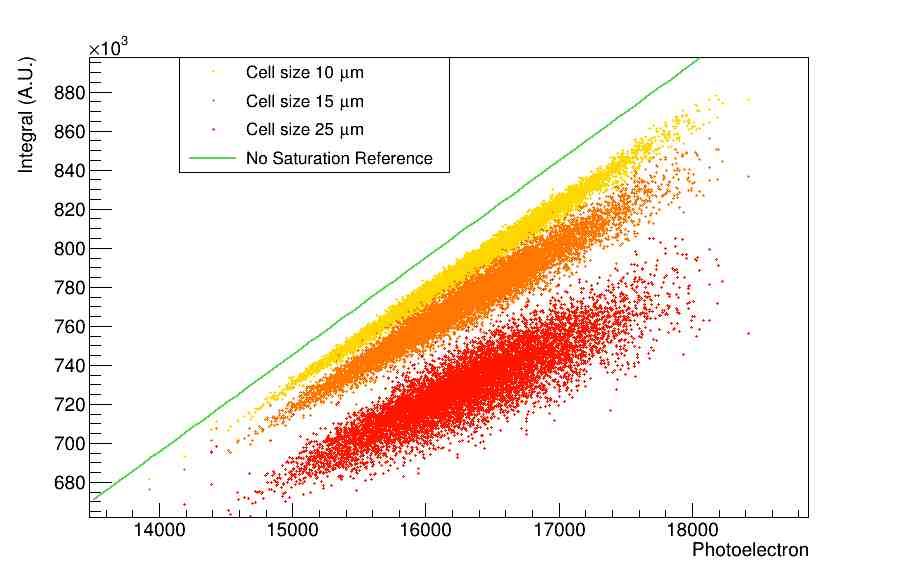
\includegraphics[width=.7\textwidth]{IMG/Sat_Ev_40GeV_scin}}
	\caption{Saturation events.}
	\label{fig:perc_sat}
\end{figure}

As can be seen, the occupancy effect in our conditions is consistent. To mitigate this problem an analytical correction can be performed through the formula:
\begin{equation}
	N_{fired}=N_{cells} \cdot \left[ 1 - \exp\left(-\frac{N_{p.e.}}{N_{cells}}\right)\right]
\end{equation}

therefore the correction has been applied modifying the integral values such as:
\begin{equation}
	I_{corr} = - A N_{cells} \left[ \ln\left(1 - \frac{I}{A N_{cells}}\right) \right]
\end{equation}

The results obtained can be visualized in figure \ref{fig:sat_corr} where are compared the data from SiPM with cell size of $10\ \mu m$ with and without analytical correction.


\begin{figure}
	\centering
	\subfloat[][$C$ signals fibres.]{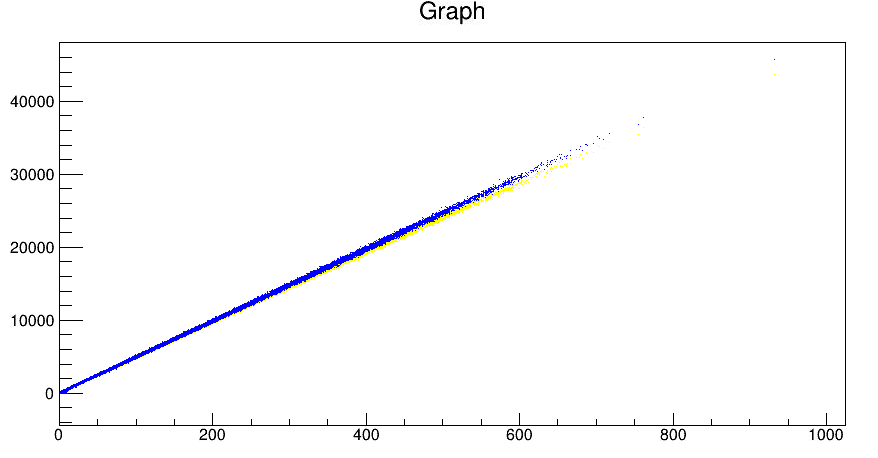
\includegraphics[width=.7\textwidth]{IMG/Corr_40GeV_fib_cher}}\\
	\subfloat[][$S$ signals fibres.]{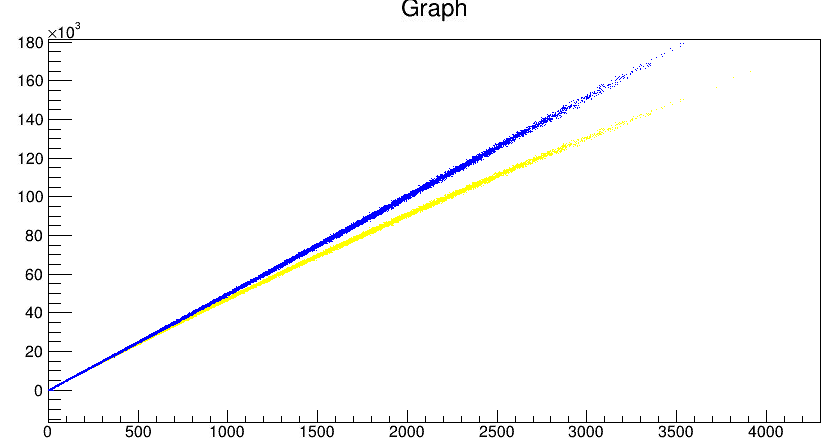
\includegraphics[width=.7\textwidth]{IMG/Corr_40GeV_fib_scin}}\\
	\subfloat[][$C$ signals events.]{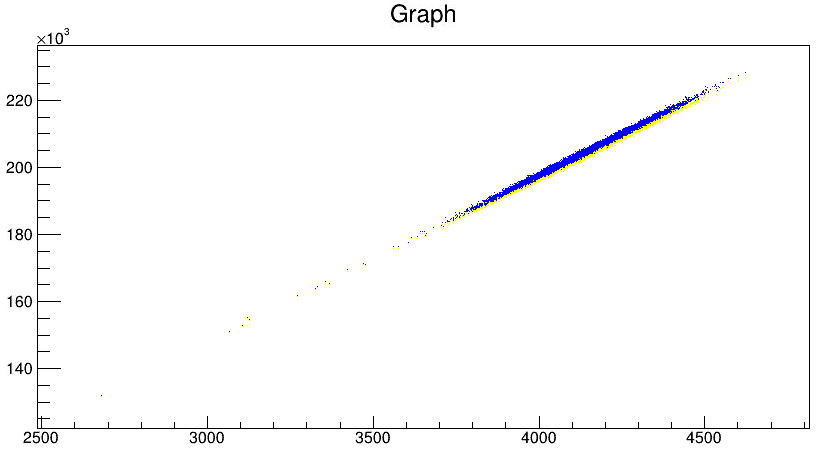
\includegraphics[width=.7\textwidth]{IMG/Corr_40GeV_ev_cher}} \\
	\subfloat[][$S$ signals events.]{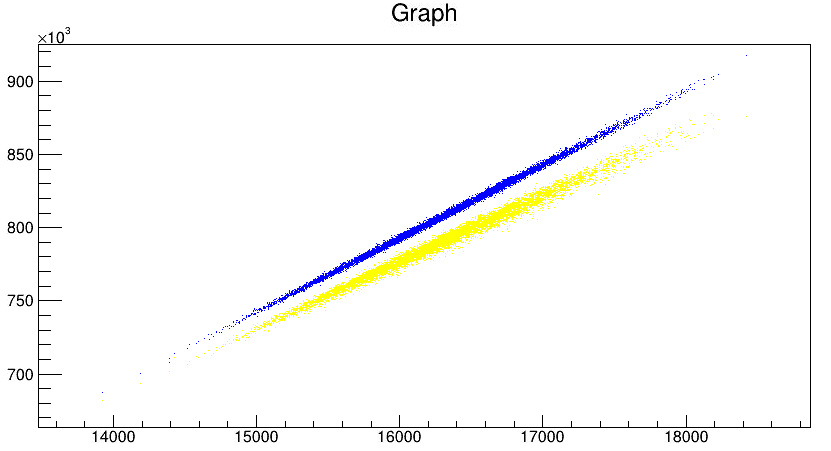
\includegraphics[width=.7\textwidth]{IMG/Corr_40GeV_ev_scin}}
	\caption{Saturation with correction.}
	\label{fig:sat_corr}
\end{figure}

The discrepancy from the no saturation reference quantifies the effect of the occupancy when performing the energy reconstruction task. The percentage difference has been evaluated through the formula $\frac{E_{NoSat}-E}{E_{NoSat}}$, and the value obtained fill the histograms in figure \ref{fig:perc_sat}.\\
After applying the analytical correction a clear improvement is show in figures \ref{fig:sat_corr_perc}.\\

\begin{figure}
	\centering
	\subfloat[][$C$ signals.]{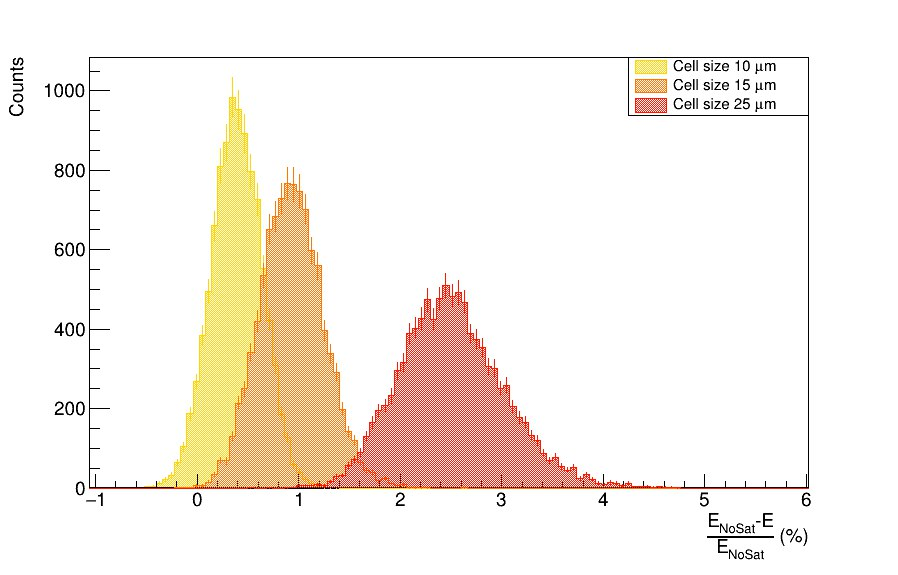
\includegraphics[width=.7\textwidth]{IMG/PercEnergy_40GeV_cher.jpg}} \\
	\subfloat[][$S$ signals.]{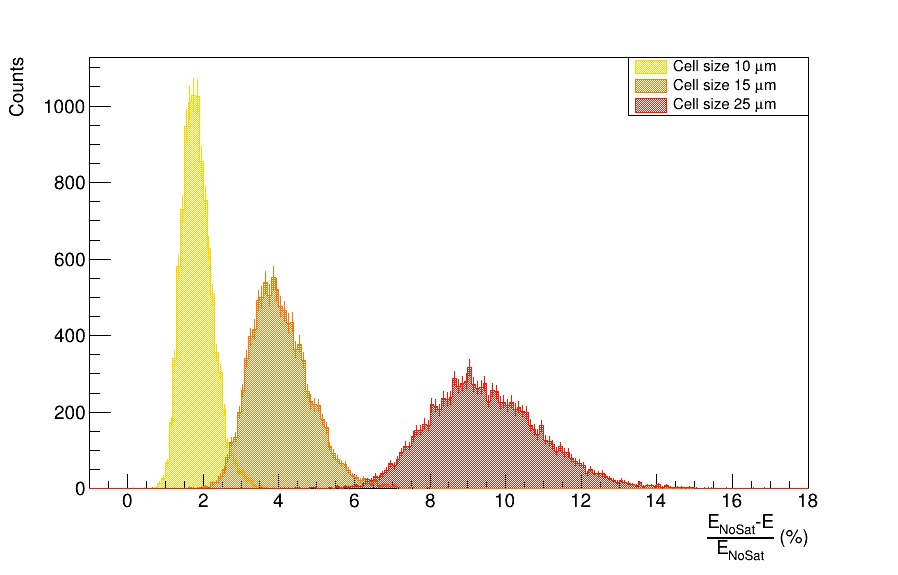
\includegraphics[width=.7\textwidth]{IMG/PercEnergy_40GeV_scin.jpg}}
	\caption{Percentage discrepancy.}
	\label{fig:sat_events}
\end{figure}

\begin{figure}
	\centering
	\subfloat[][$C$ signals.]{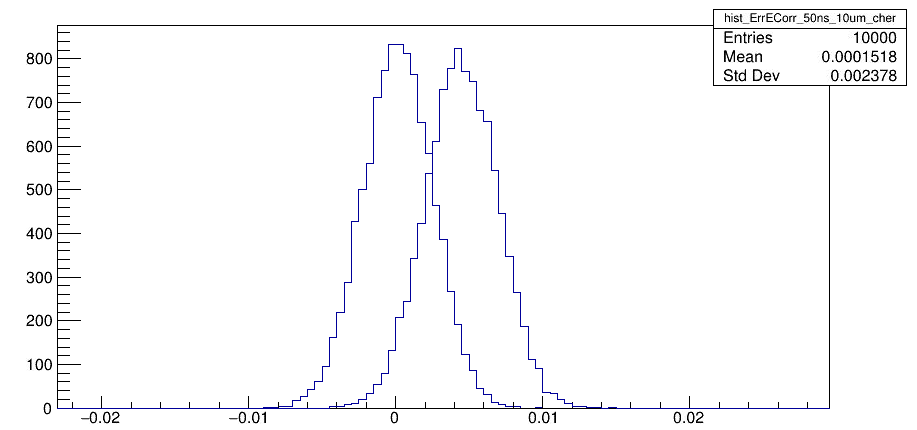
\includegraphics[width=.7\textwidth]{IMG/CorrPerc_40GeV_cher}} \\
	\subfloat[][$S$ signals.]{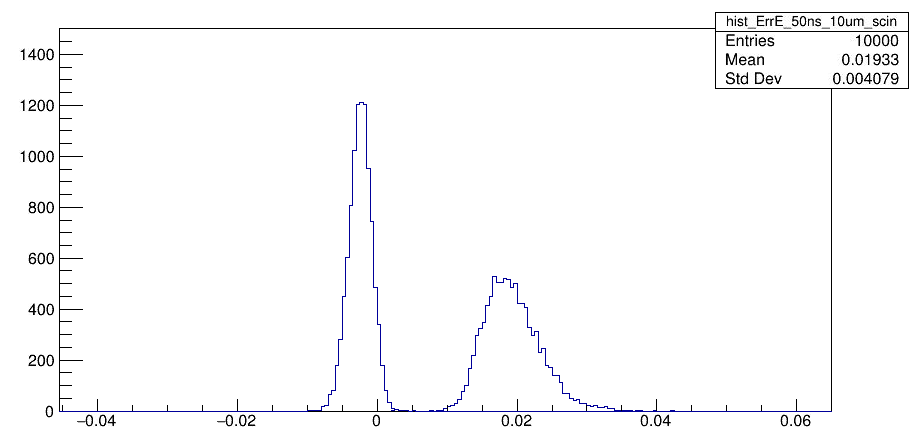
\includegraphics[width=.7\textwidth]{IMG/CorrPerc_40GeV_scin}}
	\caption{Percentage discrepancy with correction.}
	\label{fig:sat_corr_perc}
\end{figure}

This whole process has been performed simulating electrons with energies of $20,\ 40,\ 60,\ 80\ GeV$. Mean and standard deviation of the gaussian fit applied on the percentage discrepancy have been recorded and the obtained plots are shown in figure \ref{fig:sat_vs_E}.\\

\begin{figure}
	\centering
	\subfloat[][$C$ signals.]{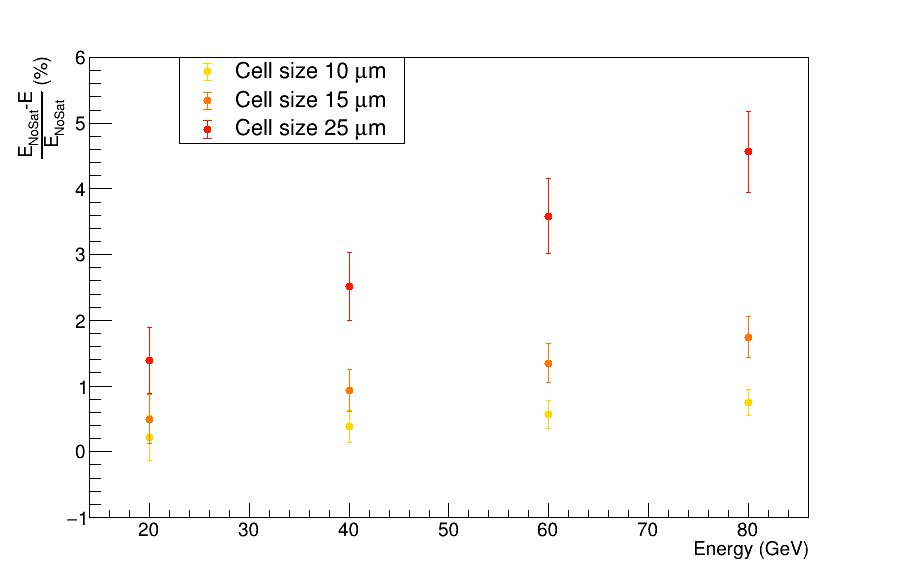
\includegraphics[width=.7\textwidth]{IMG/PercEnergy_cher}} \\
	\subfloat[][$S$ signals.]{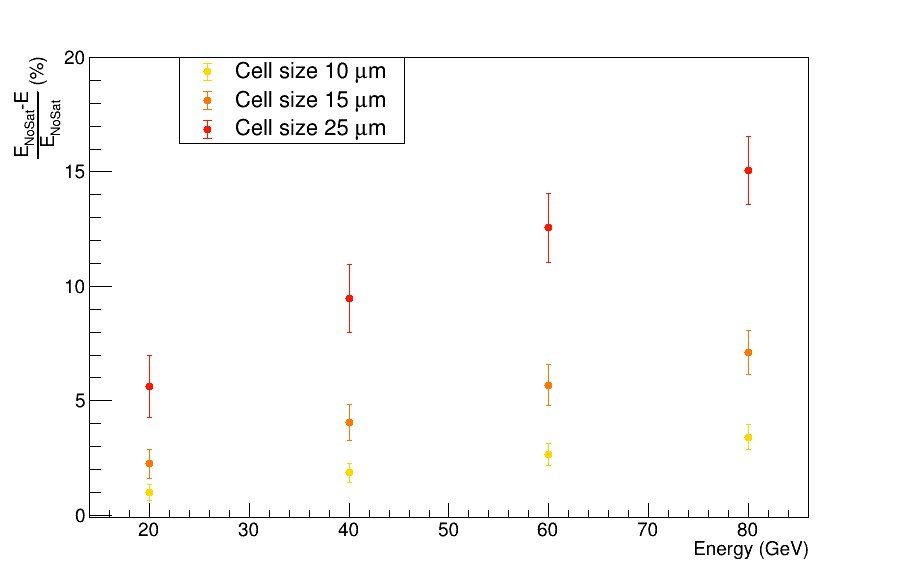
\includegraphics[width=.7\textwidth]{IMG/PercEnergy_scin}}
	\caption{Percentage discrepancy versus energy.}
	\label{fig:sat_vs_E}
\end{figure}

\subsection{Energy resolution} \label{subsec:E_res}
The first step to study the energy resolution is to calibrate the full simulation.\\
Dual-readout calorimeters are typically calibrated at the electromagnetic scale. This is specially useful in a leptonic collider because, having easily access to electrons and positrons, the calorimeter can be calibrated precisely during all the life of the experiment.\\

The calibration has been performed on $40\ GeV$ electrons applying the one-suppression already introduce un paragraph \ref{subsec:Sim_SiPM}. $10000$ events with single $40\ GeV$ electrons have been fired from the interaction point obtaining the charge integral distributions for scintillation and Cherenkov signals shown in figure \ref{fig:int_dist}. The calibration constants obtained to transform these histograms in energy distributions centered around $40\ GeV$ are: $k_S = 4.998 \times 10^{-5}$ and $k_C = 2.023 \times 10^{-4}$.\\
Two analogue calibration constants have been obtained starting from the number of photoelectrons distribution with values of:  $k_{pe,S} = 2.48 \times 10^{-3}$ and $k_{pe,C} = 1.00 \times 10^{-2}$.\\

\begin{figure}
	\centering
	\subfloat[][$C$ signals.]{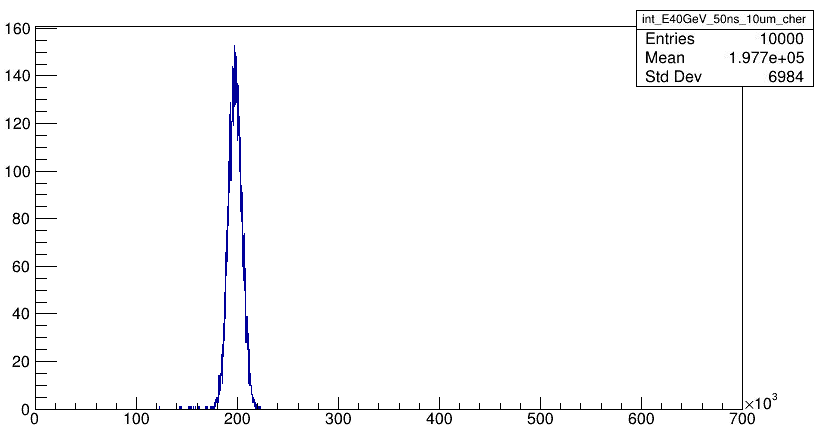
\includegraphics[width=.7\textwidth]{IMG/Intdist_40GeV_cher_cal}} \\
	\subfloat[][$S$ signals.]{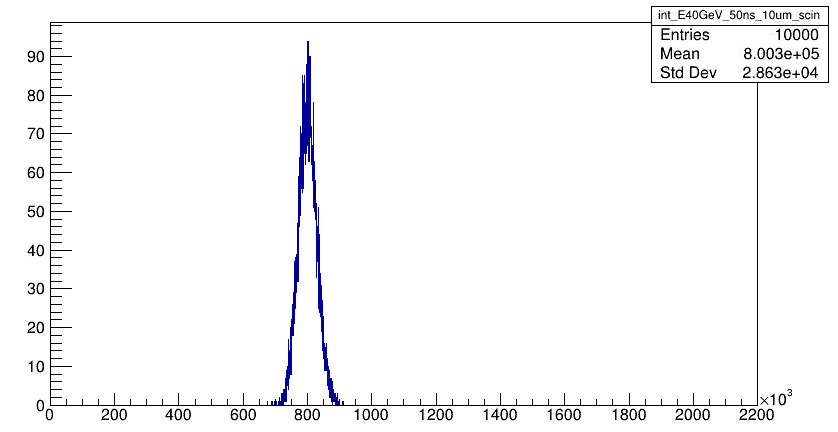
\includegraphics[width=.7\textwidth]{IMG/Intdist_40GeV_scin_cal}}
	\caption{Integral distrib.}
	\label{fig:int_dist}
\end{figure}

Starting from these calibration constant, the energy distributions can be obtained from the number of p.e. (pre SiPM digitization simulation) of from the charge integral (post SiPM digitization simulation). The two types of distribution are compared in figure \ref{fig:cfr_e_dist}.\\
As expected, the energy distributions obtained from the charge integrals are wider due to the introduction of the electronic noise. However, the effect is minimal considering the fact that in each event hundreds of SiPMs are active and the white noise has mean zero.\\

\begin{figure}
	\centering
	\subfloat[][$C$ signals.]{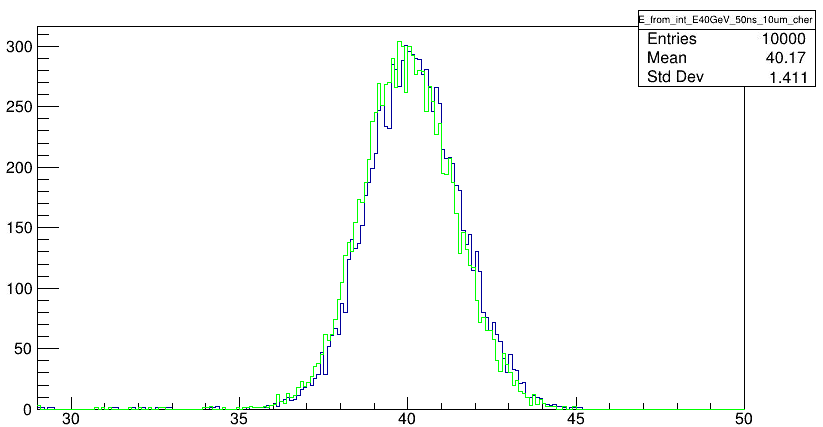
\includegraphics[width=.7\textwidth]{IMG/E_hist_cfr_cher}} \\
	\subfloat[][$S$ signals.]{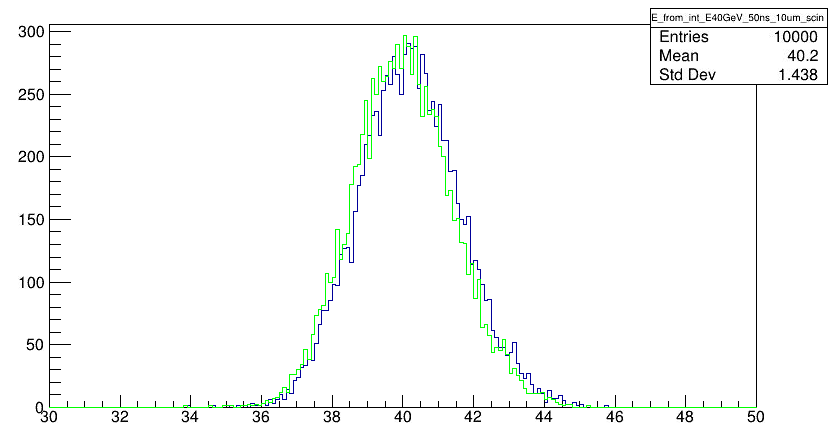
\includegraphics[width=.7\textwidth]{IMG/E_hist_cfr_scin}}
	\caption{Integral distrib.}
	\label{fig:cfr_e_dist}
\end{figure}

The energy distributions have been fitted with a Gaussian function to obtain mean, standard deviation e respective errors. Doing this with different primary electron energies the energy resolution can be studied. Mean and standard deviation are listed in tables \ref{tab:e_res_int} \ref{tab:e_res_pe}.\\
Then fitting the $\sigma/E$ values in the energy range $20-80\ GeV$ can be seen there is a good agreement with the functions:
\begin{equation}
	\frac{\sigma}{E} = \frac{A_1}{\sqrt{E}} + B_1 \qquad \text{or} \qquad \frac{\sigma}{E} = \frac{A_2}{\sqrt{E}} \oplus B_2
\end{equation} 
as shown in figure \ref{fig:sigma_su_e}. The plots also show the loss of resolution with the introduction of the SiPM digitization software.\\

\begin{table}
	\centering
	\begin{tabular}{lccc}
		\toprule
		& True Energy	(GeV) & Mean Energy (GeV) & Standard Deviation (GeV) \\
		\midrule
		\textbf{Scintillation} &	$20$ 	& $19.90$ & $0.95$ \\
		& $40$ 	& $40.20$ & $1.44$ \\
		& $60$ 	& $60.65$ & $1.85$ \\
		& $80$ 	& $81.18$ & $2.26$ \\
		\midrule
		\textbf{Cherenkov} & $20$ 	& $19.88$ & $0.95$ \\
		& $40$ 	& $40.16$ & $1.42$ \\
		& $60$ 	& $60.61$ & $1.73$ \\
		& $80$ 	& $81.12$ & $2.08$ \\
		\bottomrule
	\end{tabular}
	\caption{Sigmas}
	\label{tab:e_res_int}
\end{table}

\begin{table}
	\centering
	\begin{tabular}{lccc}
		\toprule
		& True Energy	(GeV) & Mean Energy (GeV) & Standard Deviation (GeV) \\
		\midrule
		\textbf{Scintillation} &	$20$ 	& $19.82$ & $0.92$ \\
		& $40$ 	& $40.00$ & $1.39$ \\
		& $60$ 	& $60.28$ & $1.78$ \\
		& $80$ 	& $81.58$ & $2.16$ \\
		\midrule
		\textbf{Cherenkov} & $20$ 	& $19.76$ & $0.92$ \\
		& $40$ 	& $40.01$ & $1.36$ \\
		& $60$ 	& $60.40$ & $1.66$ \\
		& $80$ 	& $81.86$ & $1.91$ \\
		\bottomrule
	\end{tabular}
	\caption{Sigmas}
	\label{tab:e_res_pe}
\end{table}

\begin{figure}
	\centering
	\subfloat[][$C$ signals.]{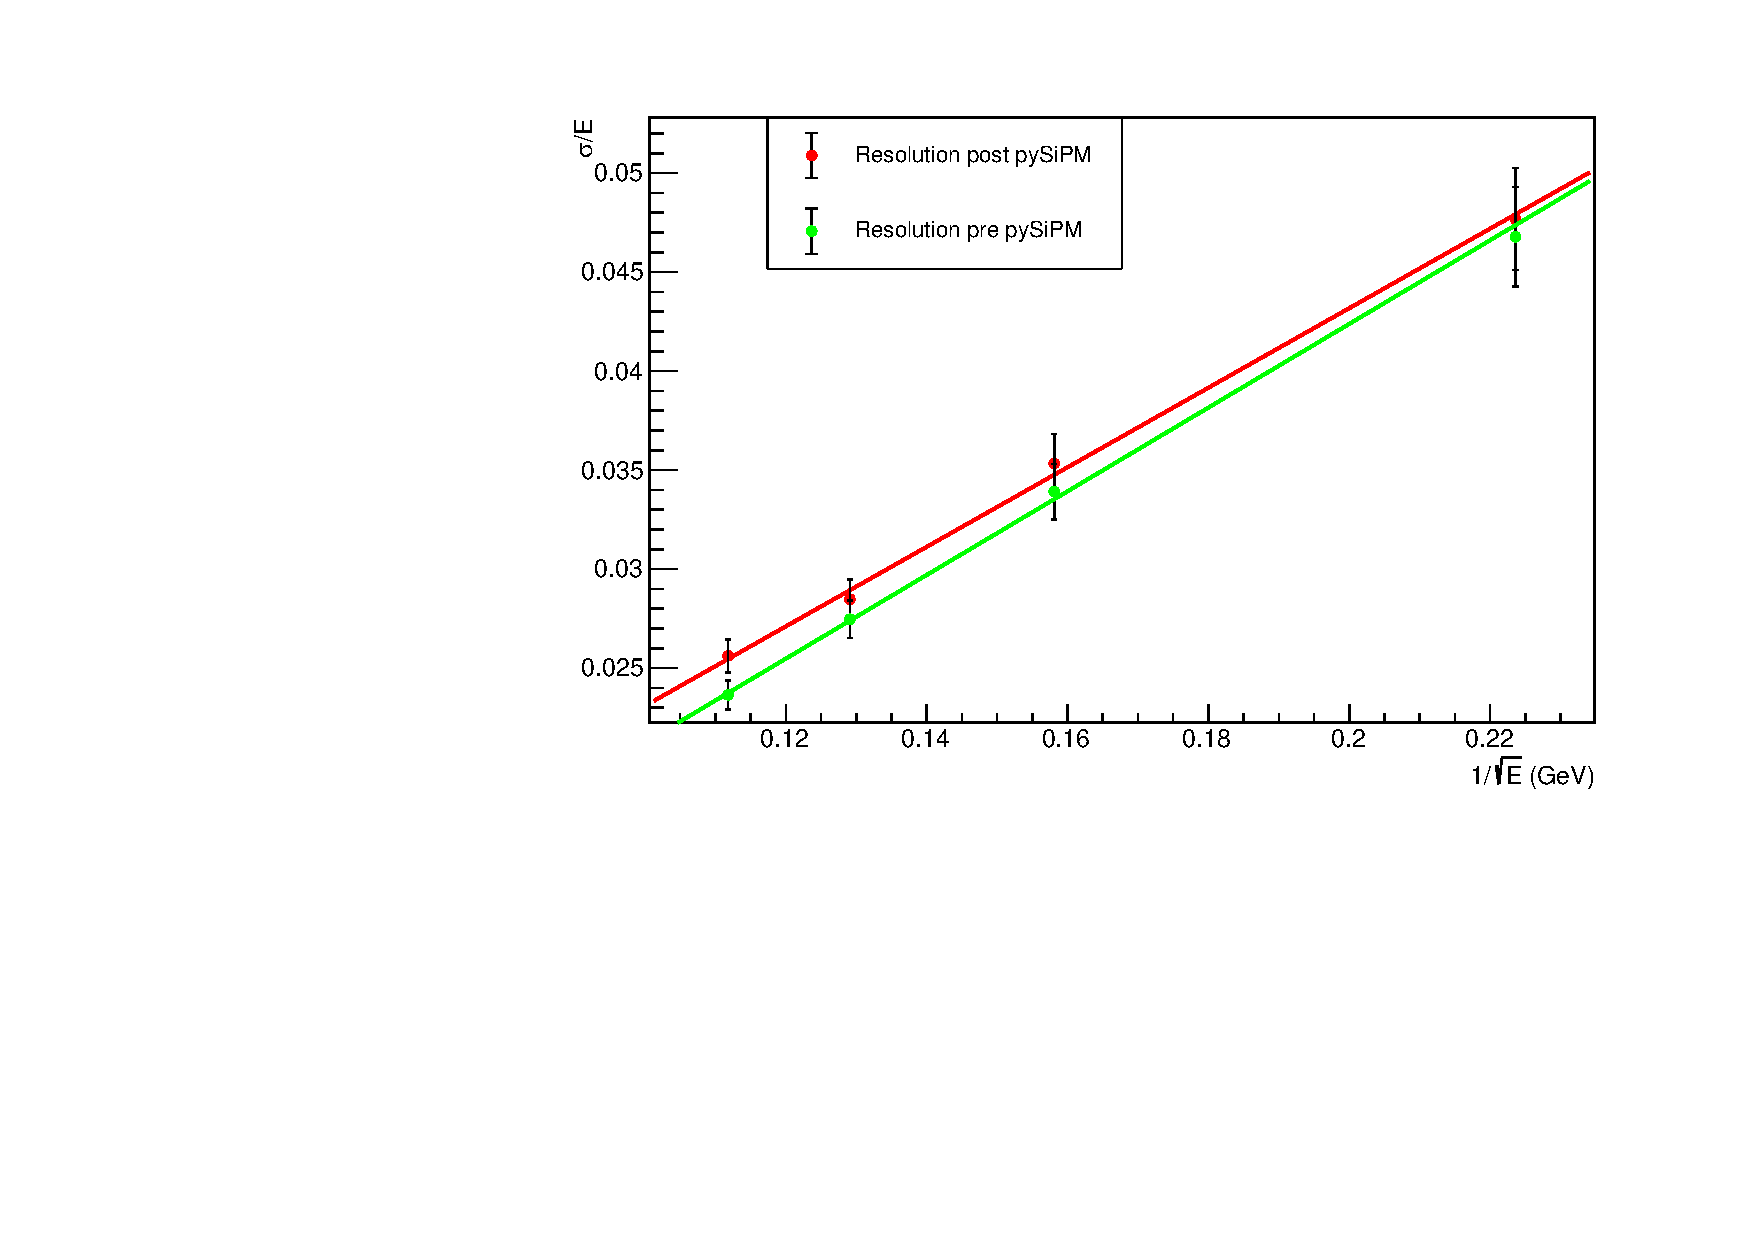
\includegraphics[width=.7\textwidth]{IMG/Res_cher}} \\
	\subfloat[][$S$ signals.]{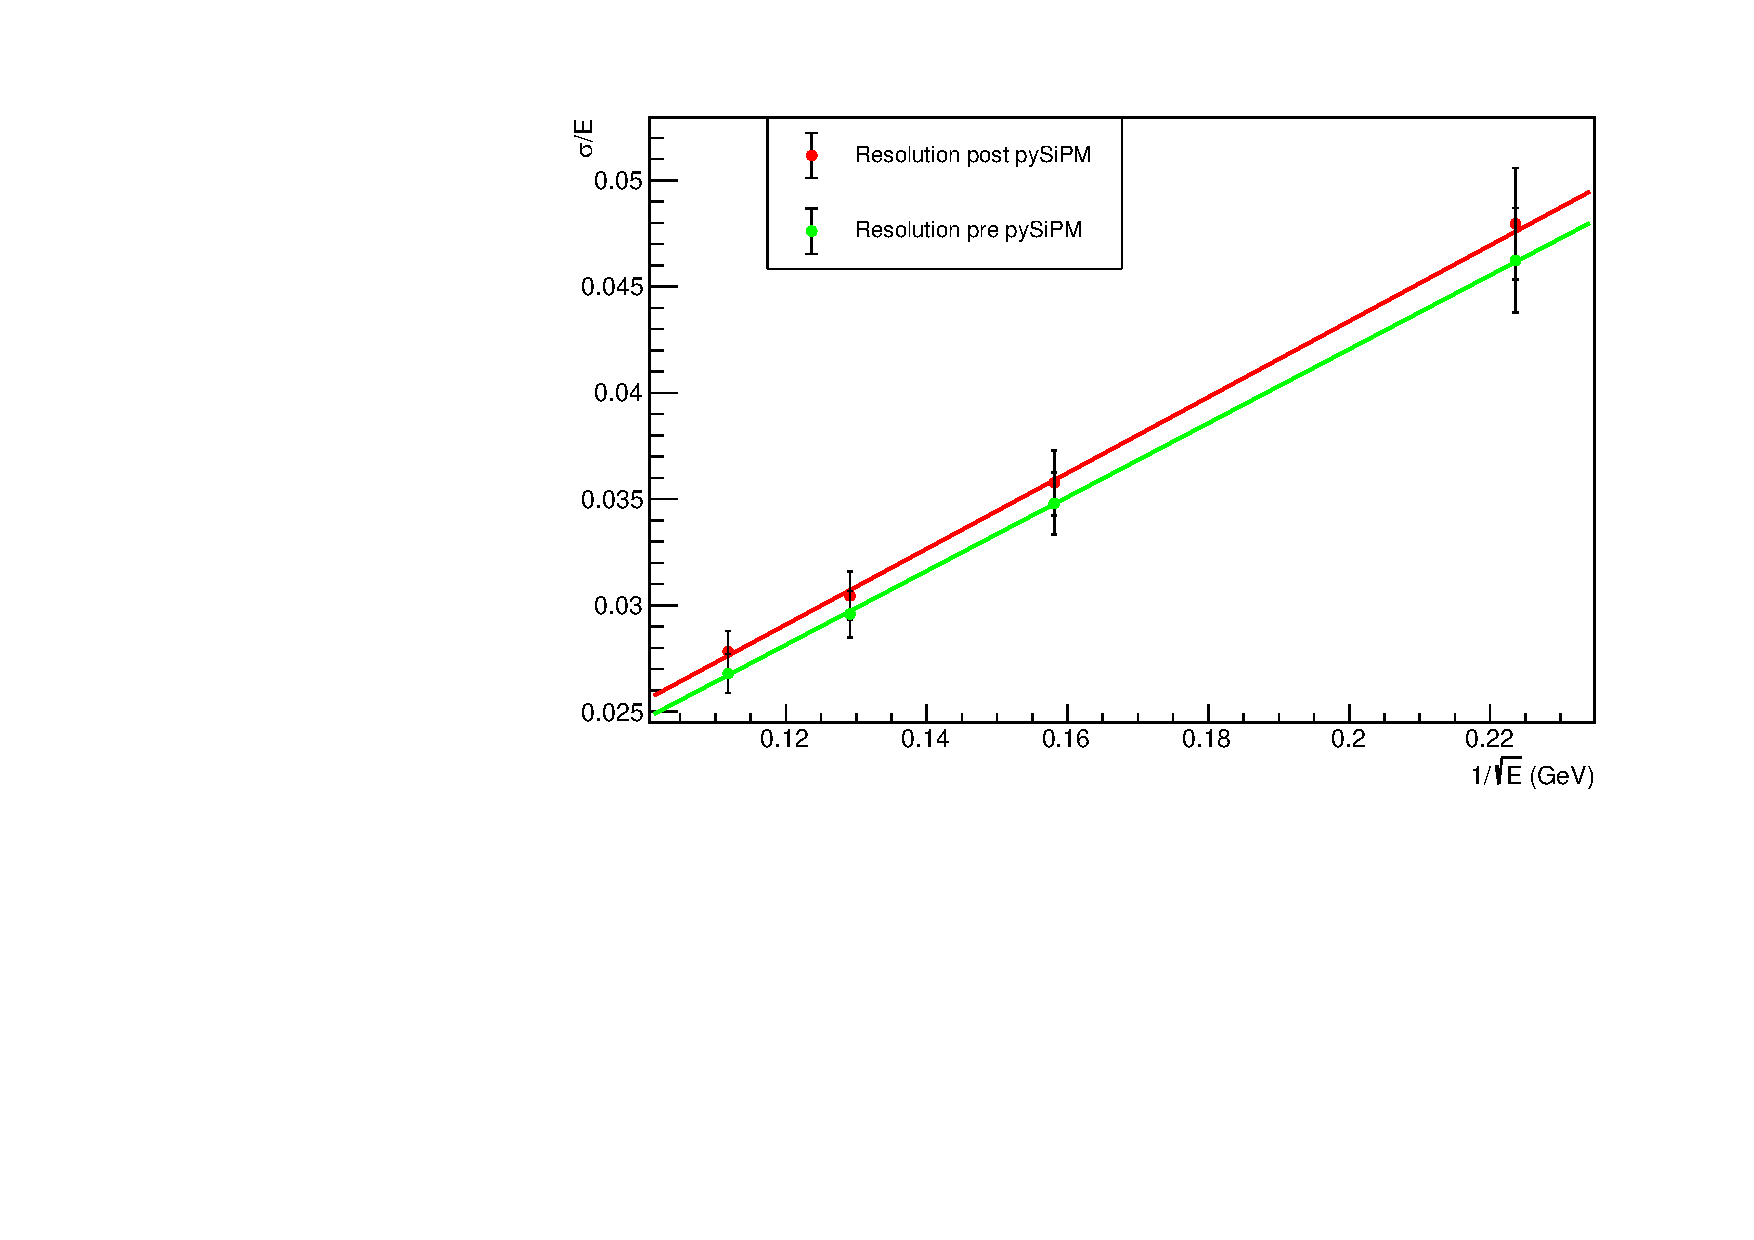
\includegraphics[width=.7\textwidth]{IMG/Res_scin}}
	\caption{Integral distrib.}
	\label{fig:sigma_su_e}
\end{figure}

\section{Neural Network: Particle ID on waveform} \label{sec:NN_waveform}
aaa

\subsection{Configuration}
aaa

\subsection{Performances}
aaa

\section{Neural Network: Particle ID on imaging} \label{sec:NN_img}
aaa

\subsection{Configuration}
aaa

\subsection{Performances}
aaa